\section{Amodal Completion}
\seclabel{amodalCompletion}
\setlength{\epigraphwidth}{.9\textwidth}
\epigraph{``Almost \textit{nothing} is visible in its entirety, yet almost \textit{everything} is perceived as a whole and complete"}{\textit{Stephen Palmer}}

Classic computer vision approaches have traditionally been impoverished by trying to explain just what we see in an image. For years, standard benchmarks have focused on explaining the visible evidence in the image - not the world behind it. For example, the well-studied task of predicting the bounding box around the visible pixels of an object has been the goal of current object detection systems. As humans, not only can we perceive the visible parts of the chair depicted in \figref{fig1}, we can confidently infer the full extent of the actual chair.

This representation of objects, that humans can effortlessly perceive, is significantly richer than what current systems are capable of inferring. We take a step forward towards achieving similar levels of understanding by attacking the task of perceiving the actual extent of the object, which we denote as \textit{amodal completion}. The amodal representation of objects enables us to leverage additional scene information such as support relationships, occlusion orderings etc. For example, given the amodal and visible extents of two neighboring objects in the image, one can figure out if one is occluded by the other. Explicitly modeling amodal representations also allow us to implicitly model occlusions patterns rather than trying to ``explain them away" while detecting objects. As described in \secref{sizeconstancy}, we can use these representations to infer real world object sizes and their relative depths just from images.

The primary focus of object recognition systems \cite{girshick2013rich,felzens_latent_pami10} has been to localize and identify objects, despite occlusions, which are usually handled as noise. Several recently proposed recognition systems do explicitly model occlusion patterns along with detections and provide a mechanism for obtaining amodal extent of the object \cite{ghiasi2014parsing, xiang_cvpr15, zia2014towards}. However, these approaches have been shown to work only on specific categories and rely on available shape models or depth inputs, for learning to reason over occlusions. In contrast, we aim to provide a generic framework that is not limited by these restrictions. Our proposed framework is described below.

\subsection{Learning to Predict Amodal Boxes}
Given a candidate visible bounding box, we tackle the task of amodal completion -- the input to our system is some modal bounding box (\eg obtained via a detection system) and we aim to predict the amodal extent for the object. We frame this task as predicting the amodal bounding box, which is defined as  the bounding box of an object in the image plane if the object were completely visible, \ie if inter-object occlusions and truncations were absent. The problem of amodal box prediction can naturally be formulated as a regression task - given a noisy modal bounding box of an object we regress to its amodal bounding box coordinates. The amodal prediction system is implicitly tasked with learning common occlusion/truncation patterns and their effects on visible object size. It can subsequently infer the correct amodal coordinates using the previously learned underlying visual structure corresponding to occlusion patterns. For example, the learner can figure out that chairs are normally vertically occluded by tables and that it should extend the bounding box vertically to predict the full extent of the chair.

Let $b = (x,y,w,h)$ be a candidate visible (or modal) bounding box our amodal prediction system receives ($(x,y)$ are the co-ordinates of the top-left corner and $(w,h)$ are the width and height of the box respectively) and $b^* = (x^*,y^*,w^*,h^*)$ be the amodal bounding box of the corresponding object, our regression targets are $(\frac{x-x^*}{w},\frac{y-y^*}{h},\frac{(x+w)-(x^*+w^*)}{w},\frac{h-h^*}{h})$. Our choice of targets is inspired by the fact that for the $y$ dimension, the height and bottom of the box are the parameters we actually care about (see \secref{sizeconstancy}) whereas along the $x$ dimension the left co-ordinate is not necessarily more important than the right.

\paragraph{Learning:} We use a Convolutional Neural Network (CNN) \cite{neocognitron,Lecun89} based framework to predict the co-ordinates of the amodal bounding box. The hypothesis is that the amodal prediction task can be reliably addressed given just the image corresponding to the visible object region -- seeing the left of a car is sufficient to unambiguously infer the full extent without significantly leveraging context. Based on this observation, we extract from input image $I$, the region corresponding to the detection box $b$ and train the CNN using targets derived as above from the amodal box $b^*$. We impose an $L_2$ penalty on the targets and regress from the extracted CNN image features to the targets. We initialize our model using the AlexNet \cite{krizhevsky2012imagenet} CNN pretrained for Imagenet \cite{imagenet_cvpr09} classification and then finetune the model specific to our task using backpropagation. Training is carried out with jittered instances of the ground truth bounding box to enable generalization from noisy settings such as detection boxes and also serve as data augmentation.

We train two variants of the above network - class-specific and class agnostic. Both these systems comprise of 5 convolutional layers followed by 3 fully-connected layers. The class-specific network has separate outputs in the last layers for different classes and is trained with positive examples from a specific class whereas the class agnostic network has a single set of outputs across all classes. Intuitively, the class-specific network learns to leverage occlusion patterns specific to a particular class (\eg chair occluded by a table) whereas the class agnostic network tries to learn occlusion patterns common across classes. Another argument for a class agnostic approach is that it is unreasonable to expect annotated amodal bounding box data for a large number of categories. A two-stage system, where we first predict the visible bounding box candidates and then regress from them to amodal boxes, enables leveraging these class agnostic systems to generalize to more categories. As we demonstrate in \secref{sizeconstancy}, this class agnostic network can be applied to novel object categories to learn object sizes.

\begin{figure}
  \centering
  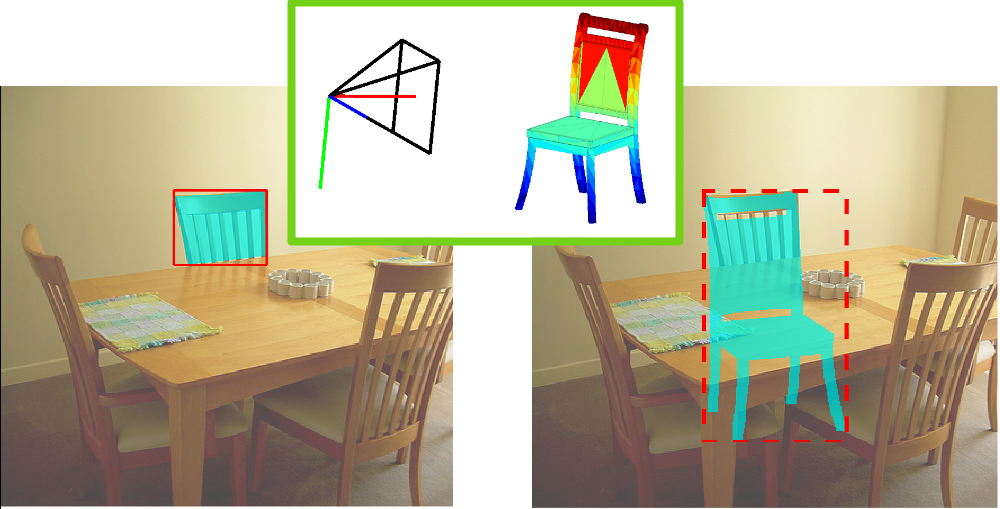
\includegraphics[width=.9\linewidth]{figures/amodal/Amodal.png}
  \caption{\figlabel{amodal} Generating amodal bounding boxes for instances in PASCAL VOC. We use the 3D models aligned to images from the PASCAL 3D+ \cite{pascal3d} and render them with their annotated 3D pose to obtain binary masks. We then use the tightest fitting bounding box around the mask as our ground truth amodal bounding box.}
\end{figure}

